\documentclass[10pt]{beamer}
\usepackage[utf8]{inputenc}

\usetheme{metropolis}

\usepackage{acronym} % \ac[p], \acl[p], \acs[p], \acf[p]
\usepackage{appendixnumberbeamer}
\usepackage{tikz}
\usetikzlibrary{positioning}

% Acronyms
% --------
\acrodef{CRDT}[CRDT]{Conflict-free Replicated Data type}
\acrodefplural{CRDT}[CRDTs]{Conflict-free Replicated Data types}

\author{Matthieu Nicolas}
\title{Efficient (re)naming in \acp{CRDT}}
\institute{
  
\includegraphics[scale=0.2]{img/ul-logo.pdf}\hspace{0.3em}University of Lorraine $|$
  
\includegraphics[scale=0.08]{img/inria-logo.pdf}\hspace{0.3em}COAST team
  \\
  \textbf{Supervised by} Gérald Oster and Olivier Perrin
  }
\begin{document}

\begin{frame}[t,plain]
  \maketitle
\end{frame}

% \begin{frame}{\acfp{CRDT}}
%   \begin{itemize}
%     \item A family of data structures
%     \item Behave like traditional ones...
%     \item ... but designed for distributed usage
%   \end{itemize}
% \end{frame}

% \begin{frame}{String}
%   \begin{itemize}
%     \item Example with two concurrent insert (operations do not commute)
%   \end{itemize}
% \end{frame}

% \begin{frame}{LogootSplit}
%   \begin{itemize}
%     \item Example with two concurrent insert (operations commute)
%     \item Work by attaching identifiers to each block of text
%   \end{itemize}
% \end{frame}

% \begin{frame}{But identifier size keeps increasing}
%   \begin{itemize}
%     \item Example using a split
%     \item Has to increase size of identifier to comply to the order
%     \item Dense set
%   \end{itemize}
% \end{frame}

\begin{frame}{\acfp{CRDT}}
  \begin{columns}
    \begin{column}{0.6\textwidth}
      \begin{tikzpicture}

        \node (A) at (0, 0) {
\includegraphics[scale=0.035]{img/userA.pdf}};
        \node[below=3pt of A] {\textbf{Alice}};
        \node<1>[above=3pt of A] {
\includegraphics[scale=0.4]{img/doc.pdf}};
        \node<2-4>[above=3pt of A] {
\includegraphics[scale=0.4]{img/docA.pdf}};
        \node<5->[above=3pt of A] {
\includegraphics[scale=0.4]{img/docABC.pdf}};

        \node (B) at (-2, -3) {
\includegraphics[scale=0.035]{img/userB.pdf}};
        \node[below=3pt of B] {\textbf{Bob}};
        \node<1-2>[left=3pt of B] {
\includegraphics[scale=0.4]{img/doc.pdf}};
        \node<3>[left=3pt of B] {
\includegraphics[scale=0.4]{img/docA.pdf}};
        \node<4>[left=3pt of B] {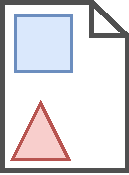
\includegraphics[scale=0.4]{img/docAB.pdf}};
        \node<5->[left=3pt of B] {
\includegraphics[scale=0.4]{img/docABC.pdf}};

        \node (C) at (2, -3) {
\includegraphics[scale=0.035]{img/userC.pdf}};
        \node[below=3pt of C] {\textbf{Carl}};
        \node<1-2>[right=3pt of C] {
\includegraphics[scale=0.4]{img/doc.pdf}};
        \node<3>[right=3pt of C] {
\includegraphics[scale=0.4]{img/docA.pdf}};
        \node<4>[right=3pt of C] {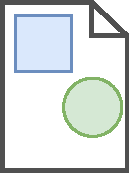
\includegraphics[scale=0.4]{img/docAC.pdf}};
        \node<5->[right=3pt of C] {
\includegraphics[scale=0.4]{img/docABC.pdf}};

        \draw[shorten >=3pt, shorten <=3pt]
          (A) to[bend right] (B)
          (B) to[bend right] (C)
          (C) to[bend right] (A);

        \node<2>[below left=-25pt and 5pt of A] {
\includegraphics[scale=0.4]{img/updateA.pdf}};
        \node<2>[below right=-25pt and 5pt of A] {
\includegraphics[scale=0.4]{img/updateA.pdf}};

        \node<4>[below right=-4pt and 1pt of B] {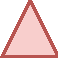
\includegraphics[scale=0.4]{img/updateB.pdf}};
        \node<4>[above left=1pt and -15pt of B] {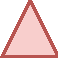
\includegraphics[scale=0.4]{img/updateB.pdf}};

        \node<4>[below left=-4pt and 1pt of C] {
\includegraphics[scale=0.4]{img/updateC.pdf}};
        \node<4>[above right=1pt and -15pt of C] {
\includegraphics[scale=0.4]{img/updateC.pdf}};
      \end{tikzpicture}
    \end{column}
    \begin{column}{0.4\textwidth}
      \begin{itemize}
        \item Replicated data structure
        \item<2-> Updates performed without coordination
        \item<3-> Eventual consistency
      \end{itemize}
    \end{column}
  \end{columns}
\end{frame}

\begin{frame}{Identifier-based \acp{CRDT}}
  \begin{block}{Identifiers}
    \begin{itemize}
      \item Attached to elements to handle concurrent updates
      \item Have to comply to several constraints
      \begin{itemize}
        \item<2-> Order relation
        \item<3-> Causality relation
        \item<4-> ...
      \end{itemize}
    \end{itemize}
  \end{block}
  \begin{alertblock}{Limits}<5->
    \begin{itemize}
      \item Unbounded size of identifiers
      \item Efficiency decreasing over time
    \end{itemize}
  \end{alertblock}
\end{frame}

\begin{frame}{Research questions}
  \begin{block}{Can we propose}
    \begin{itemize}
      \item more efficient identifiers given several constraints ?
      \item mechanisms to rename identifiers ?
    \end{itemize}
  \end{block}
\end{frame}

% NOTE: Put it after the "Thanks" slide ?
\begin{frame}{Next step}
  \begin{itemize}
    \item Build taxonomy of constraints on identifiers and of current solutions
  \end{itemize}
\end{frame}

%\begin{frame}{Example}
%  \begin{center}
%    \includegraphics[scale=0.25]{path/to/fig}
%  \end{center}
%\end{frame}

\begin{frame}[standout]
  Thanks for your attention, any questions?
\end{frame}

\begin{frame}[allowframebreaks]{References}
	\bibliography{biblio}
	\bibliographystyle{abbrv}
\end{frame}

\end{document}
